\section{Evaluation}
\label{sec:eval}
The evaluation measures proof and storage costs, the admission boundary, the amount channel, and fleet escrow. The build pins Circom 2.1.9, its first optimization level, BN254 and the bundled circuit library. The host is an Apple M4 Mac with 16 GiB memory. The payload includes \CircuitMains{} compiled mains, \ApplicationKeys{} application verification keys with \PublicCoordinates{} public inputs, and \ProofBundles{} proof bundles.

\subsection{Constraint and host costs}
\label{sec:eval-scale}

\begin{figure*}[t]
\centering
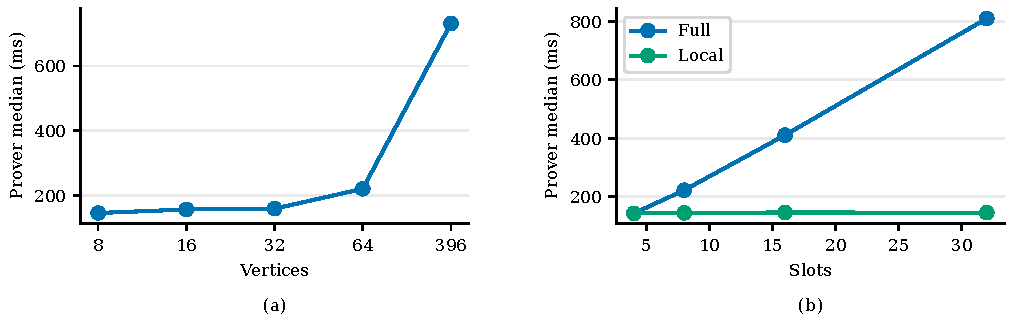
\includegraphics[width=\textwidth]{figures/fig3_scaling.pdf}
\caption{Prepared-witness component costs. (a) Vertex scaling. Error bars show symmetric half interquartile ranges. The 396-cell case uses the causal hub circuit. (b) Full and local proving replay the same opening on registered four-slot gaps.}
\label{fig:scaling}
\end{figure*}

\begin{table}[t]
\centering
\scriptsize
\setlength{\tabcolsep}{4pt}
\begin{tabular}{@{}lrrrrr@{}}
\toprule
Configuration & R1CS & Med. ms & IQR & p95 & MiB \\
\midrule
Prepared $N=8$ & 32,947 & 146.8 & 3.0 & 155.3 & 44.8 \\
Prepared $N=16$ & 41,896 & 157.7 & 2.9 & 164.2 & 56.5 \\
Prepared $N=32$ & 59,785 & 160.1 & 5.4 & 170.5 & 65.4 \\
Prepared $N=64$ & 98,938 & 221.3 & 4.4 & 245.6 & 85.4 \\
Prepared $N=396$ & 356,837 & 730.7 & 30.0 & 789.6 & 427.8 \\
\midrule
Host end-to-end & 357,048 & 3,669.1 & 432.8 & 6,759.3 & 428.2 \\
\bottomrule
\end{tabular}

\caption{Historical prepared-witness scaling and paired host latency. The largest prepared circuit uses a different architecture. The host row includes witness, prove and verify.}
\label{tab:scaling}
\end{table}


The stored prepared-witness benchmarks compare four sparse vertex cases with a separate 396-cell hub design. The vertex A/A arms measure repeatability within each architecture and vertex count. The largest case recorded 8 MiB additional used swap and 307 pageouts. The local-gap relation amortizes the authenticated sibling path and reduces proving in the registered 16- and 32-slot cases. Setup and anchor enrollment are separate from these prepared-witness timings.

For the current 396-cell update, each of \HostTrials{} host trials generates a native witness, proves, and verifies the same trial. The witness and prover run as macOS background-priority processes with a requested two-thread OpenMP setting. Median end-to-end latency is \HostMedian{} s (Q25--Q75 \HostQone{}--\HostQthree{} s, p95 \HostPninetyfive{} s). Peak child RSS is \HostRSS{} MiB. A separate attempt during fleet proving had \HostLoadedFailures{} failures among \HostLoadedTrials{} timed trials. The receipt retains that attempt. Device limits, ARM latency and delegated networking are outside this host measurement.

\subsection{Authenticated comparator costs}
\label{sec:eval-baselines}

\begin{table*}[t]
\centering
\scriptsize
\setlength{\tabcolsep}{4pt}
\begin{tabular}{@{}lrrrrrrrr@{}}
\toprule
Settlement arm & Rows & Store B & Prep ms & Upd B & Client ms & Admit ms & Close B & Close ms \\
\midrule
Plaintext evidence & 0 & 0 & -- & 110 & 0.02 & 0.30 & 800 & 0.02 + 0.27 \\
Online trusted source & 0 & 0 & -- & 125 & 0.16 & 0.23 & 125 & 0.05 + 0.24 \\
Factored offline $m\,2^g$ & 64 & 8,000 & 1.91 & 500 & 0.06 & 0.34 & 500 & 0.06 + 0.35 \\
Coupled offline $2^n$ & 65,536 & 8,192,000 & 7,678.50 & 125 & 0.02 & 0.26 & 125 & 0.02 + 0.26 \\
\midrule
TollVeil Taiwan & -- & -- & -- & 1,103 & 1,722.5 + 607.0 & 10.11 & 1,029 & see Table~\ref{tab:corridors} \\
TollVeil Rome & -- & -- & -- & 1,106 & 4,475.7 + 1,466.7 & 8.23 & 1,034 & see Table~\ref{tab:corridors} \\
\bottomrule
\end{tabular}
\par\smallskip\begin{tabular}{@{}llr@{}}\toprule
Related system & Measured operation and trust boundary & Reported cost \\
\midrule
PrETP~\cite{pretp2010} & reimplemented eight-segment commitment and audit & 19.03 ms \\
ERP~\cite{desmet2024} / Bulletproofs~\cite{bulletproofs2018} & standalone 64-bit range-proof reference & 672 B \\
FairStream~\cite{fairstream2023} & pessimistic proof of misbehavior, modeled chain gas & 112,176 gas \\
CAPE~\cite{cape2025} & reimplemented private channel update proof & 36.834 s \\
FairRelay~\cite{fairrelay2026} & proof of forwarding circuit & 6.014 s \\
MicroNova~\cite{micronova2025} & incremental fold and final compression & 170.7 / 5,209.6 ms \\
\bottomrule\end{tabular}
\caption{Authenticated settlement costs and related primitive references. The signed arms share a synthetic 16-slot task, and the TollVeil rows use the indicated corridor inputs. The offline catalogs assume route foreknowledge. Signed close reports client and charger medians separately.}
\label{tab:baselines}
\end{table*}


\begin{figure*}[t]
\centering
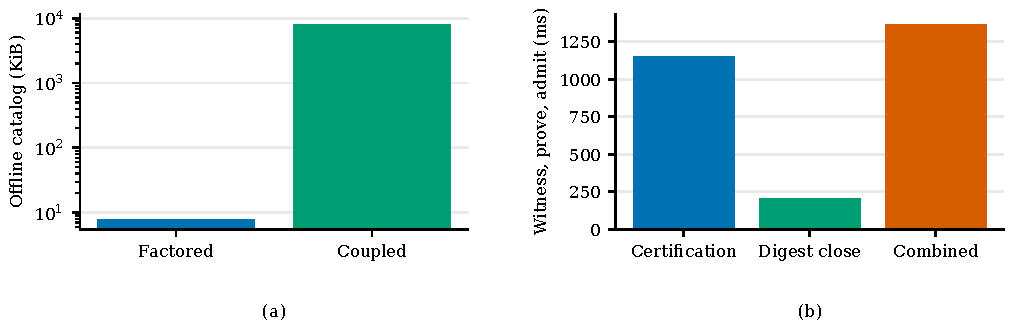
\includegraphics[width=\textwidth]{figures/fig6_baselines_close.pdf}
\caption{(a) Persistent catalog storage on the 16-slot signed fixtures. (b) Wall stages for a gap digest close, including the separate authoritative certification. The scope of each panel determines its units.}
\label{fig:baseline-close}
\end{figure*}

The signed prototype arms authenticate an opening and compute a safe release and terminal charge. The plaintext arm reveals opened edges to the charger. The online trusted source computes and signs the bound after receiving the authorized mask. Offline programs sign a catalog before the trip under the stronger assumption that the source knows the route. A factored catalog stores $m\,2^g$ rows with independent enrolled anchors. In the coupled catalog the candidate path can cross every intermediate boundary, and the exhaustive encoding stores $2^n$ rows. The charger verifies the returned entries and the declared mask. Storage, bytes on the wire, prep, and terminal costs are separately reported. The four signed arms share one settlement objective and differ in disclosure and trust. The two proof-based rows use their own corridor inputs. The named external protocols exercise different primitives, shown in the lower panel of Table~\ref{tab:baselines} with their measurement scopes.

A complete digest close includes \GapCertifyCloseMs{} ms for the measured certification-plus-close path. The digest proof and its admission account for \GapCloseMs{} ms of that total. Figure~\ref{fig:baseline-close}(b) uses one common fault and predecessor scope. A separate component fixture satisfies the stateful requirement of at least three openings per gap. With one common predecessor, bulletin and fault, raw, stateful and digest proving took \GapMatchedRawMs{}, \GapMatchedStatefulMs{} and \GapMatchedDigestMs{} ms. These three proof times exclude admission and the prior digest certification.

\subsection{Stopping, amount disclosure, and transport}
\label{sec:eval-privacy}

\begin{figure*}[t]
\centering
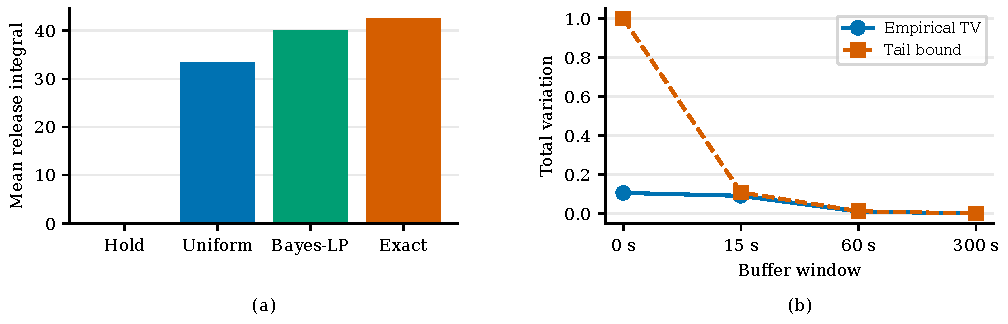
\includegraphics[width=\textwidth]{figures/fig4_privacy_net.pdf}
\caption{(a) Fixed-site utility on the constructed finite support. (b) Empirical total variation (TV) and a tail bound for two simulated delay profiles. The plotted 300-second empirical value depends on the sampled executions.}
\label{fig:privacy-net}
\end{figure*}

\begin{table}[t]
\centering
\scriptsize
\setlength{\tabcolsep}{4pt}
\begin{tabular}{@{}lrrrrr@{}}
\toprule
Cohort & Amount view & Top-1 & Bits & Group Top-1 & $>5$ pp \\
\midrule
Rome & Hold & 81.6\% & 0.0000 & 34.7\% & 0 \\
Rome & Slot 4 bucket & 81.6\% & 0.0000 & 34.7\% & 0 \\
Rome & Multi-slot bucket & 88.1\% & 0.0790 & 57.9\% & 30 \\
Rome & Exact & 98.8\% & 0.1831 & 95.8\% & 60 \\
\midrule
Taiwan & Hold & 99.8\% & 0.0000 & 99.8\% & 0 \\
Taiwan & Slot 4 bucket & 99.8\% & 0.0000 & 99.8\% & 0 \\
Taiwan & Multi-slot bucket & 99.8\% & 0.0000 & 99.8\% & 0 \\
Taiwan & Exact & 99.8\% & 0.0000 & 99.8\% & 0 \\
\bottomrule
\end{tabular}

\caption{Second-order score after observing the complete intermediate amount vector. Group Top-1 uses non-singleton groups. Exact is an unconstrained reference.}
\label{tab:privacy}
\end{table}


The Rome experiment pairs fixed late stopping with an external stopping intervention under each of two payer information sets. The causal arm equates same-site observations, and the sealed arm exposes the complete history, including the route and measurement and fault state, to the payer. The terminal key contains the entry and settlement amount, at the same stop, under the fixed enrollment and bulletin scope. The four cells each cover \RomeStopSites{} decisions. External stopping shrinks \RomeStopCausal{} decisions under causal information and \RomeStopSealed{} under sealed history. In the causal row, fixed-late and externally chosen stopping yield \StopCausalLate{} and \StopCausalAny{} total release units across all sites. In the sealed row the corresponding totals are \StopSealedLate{} and \StopSealedAny{}.

The prior fits second-order transitions on the calibration vehicles in Rome and the earlier time window in Taiwan. It is normalized on the observed holdout route dictionary grouped by settlement key, including vehicle class for Taiwan. Of the Rome support, \RomePriorGroups{} non-singleton groups contain \RomePriorBlocks{} blocks. The scorer uses the same Hold, slot-four, multi-slot and Exact policies as the fleet replay. It reports full support and fleet-subset scores separately. The Taiwan holdout contains only four terminal-key groups with distinct routes, and the fleet subset contains \TaiwanFleetRouteGroups{}. This limits the amount-channel comparison on Taiwan. The 2,000-unit Rome single bucket has \RomeSingleCapViolations{} outcomes more than five percentage points above the group's prior vulnerability. The joint seven-slot release vector has \RomeMultiCapViolations{} such outcomes, and the unconstrained Exact release has \RomeExactCapViolations{}. The Taiwan bucket width is \TaiwanBucketWidth{} new Taiwan dollars (TWD). By construction, these are posterior comparisons under the stipulated model and terminal observations. The repeated \SyntheticSupport{}-history finite benchmark has a \SyntheticGain{} single-site utility gain for its linear program over its uniform bucket.

The transport model simulates two profiles with reconnection bursts and binned residual delays at fixed packet cadence, using a simplified vehicle-network methodology~\cite{tr37885}. At a 60-second window, empirical TV is \NetworkTV{} and the simultaneous tail upper bound is \NetworkBound{} under that model. The adaptive whole-view bound in Theorem~\ref{thm:priv} remains a modeling premise.

\subsection{Archived corridors and timestamp-aligned fleet credits}
\label{sec:eval-fleet}

\begin{figure*}[t]
\centering
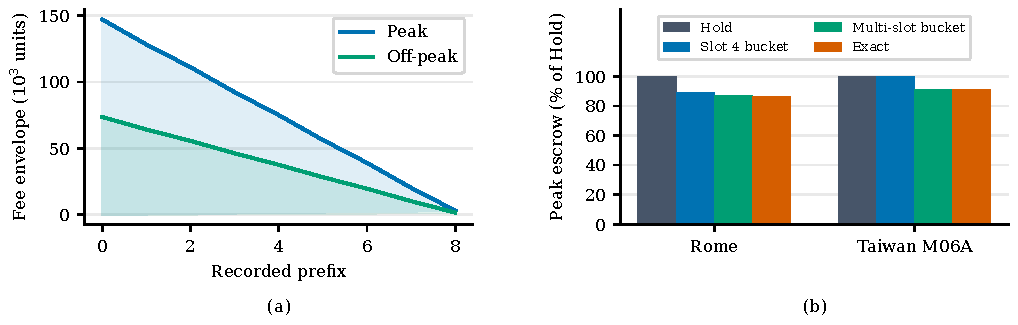
\includegraphics[width=\textwidth]{figures/fig5_real_corridors.pdf}
\caption{(a) Historical offline Rome envelope contraction across prefixes. (b) Peak locked escrow normalized to a matched Hold replay. Each Taiwan bar uses its own release policy and observed-time ledger receipt.}
\label{fig:corridors}
\end{figure*}

\begin{table}[t]
\centering
\scriptsize
\setlength{\tabcolsep}{4pt}
\begin{tabular}{@{}lrr@{}}
\toprule
Metric & Rome & Taiwan \\
\midrule
Selected proof sessions & 55 & 36 \\
Admitted proofs & 220 & 108 \\
Conservation errors & 0 & 0 \\
Update witness / prove (ms) & 4,475.7 / 1,466.7 & 1,722.5 / 607.0 \\
Close witness / prove (ms) & 4,472.3 / 1,544.8 & 1,381.6 / 595.7 \\
Update pairing / precommit (ms) & 7.90 / 8.23 & 9.49 / 10.11 \\
Close pairing / precommit (ms) & 7.75 / 8.17 & 8.63 / 9.25 \\
Update / close bytes & 1,106 / 1,034 & 1,103 / 1,029 \\
\midrule
Hold escrow peak & 588,800 & 18,176 \\
Slot 4 bucket escrow peak & 522,800 & 18,176 \\
Multi-slot bucket escrow peak & 510,800 & 16,556 \\
Exact escrow peak & 508,618 & 16,532 \\
\bottomrule
\end{tabular}

\caption{Proof-gated replays on archived routes with synthetic credentials. Bytes count serialized proof and public vector. Precommit time includes pairing and transaction work before receipt insertion.}
\label{tab:corridors}
\end{table}


The Rome release reproduces the 1,000 historical prepared blocks byte for byte from the CRAWDAD input~\cite{crawdadroma2014}. It recenters each ten-fix block, quantizes to 100 m and evaluates these route shapes over a representative 500 m Rome road-cost graph. The eligible blocks split by taxi identifier into 476 calibration, 337 holdout and 43 reserved blocks. The earlier compiled check reports \HistoricalRomePrefix{} holdout prefixes and \HistoricalSyntheticPrefix{} synthetic prefixes, including genesis. The current selected \RomeSessions{} sessions generate \RomeProofs{} proof admissions. The injected outage cases use simulated credentials and assigned masks.

The Taiwan topology is built from first detections in 08:00--08:30~\cite{taiwantdcs2019}. The held-out 08:30--09:00 slice deterministically selects \TaiwanHoldout{} trajectories supported by those \TaiwanGantries{} gantries and \TaiwanEdges{} directed edges including exit. Direct summation of the archived gantry list and the forward replay agree on \TaiwanListMatches{} trips. The fee table postdates the traces. The separate per-trip allowance diagnostic agrees on \TaiwanAllowanceMatches{} trips. Billing records with daily per-vehicle allowances are outside this comparison. The current corpus yields \TaiwanProofs{} admissions over \TaiwanSessions{} trips.

The fleet evaluation replays the same sequence of enrollment and checkpoint timestamps for each policy. Proofs are prepared in advance, so live proving and queueing delays lie outside the replay clock. Rome uses archived fix times. Taiwan uses gantry detection times with virtual exit slots at the last detection. The pool admits proofs before any credit, tracking reuse of intermediate credits separately from final refunds. The recorded peaks are \RomePeakConcurrent{} simultaneous Rome trips and \TaiwanPeakConcurrent{} Taiwan trips. A single bucketed intermediate release changes peak escrow from Hold by a reduction of \RomeSinglePeakSavings{} and \TaiwanSinglePeakSavings{}, respectively. Figure~\ref{fig:corridors}(b) compares that policy with the multi-slot and Exact arms. The local pooled balance measures internal reuse. Bank transfers lie outside this replay.
